\chapter{Control Systems}
\section{Optimal control problem}
	The optimal control problem goes back more than 300 years. From Galileo and Newton to Johann Bernoulli and Euler with the Brachistochrone problem. The goal in optimal control is to find the appropriate inputs or control law. So that the dynamic system behaves optimally, according to some criterion. 
	
	The main ingredients involved in the definition of an optimal are: a set of differential equations that describes the behavior of the system. A cost function that describes the cost of the specific trajectory integrated on the differential equations. The optimal solution will have the lowest cost possible.
	
	Optimal control problems can be mathematically defined as the cost function \eqref{eq:optimal control definition}(With boundary conditions \eqref{eq:optimal control definition state equations boundary conditions})  and the behavior of the system \eqref{eq:optimal control definition state equations}. In addition constraints can be placed on the state and inputs, as shown by \eqref{eq:optimal control definition state equations path constraints}. 
	
	\begin{equation}
		J = S[x(t_0),t_0,x(T),T] + \int_{t_0}^{T} L[x(t),u(t),t]
		\label{eq:optimal control definition}
	\end{equation}
	\begin{equation}
		\dot{x}(t) = F(x(t),u(t),t)
		\label{eq:optimal control definition state equations}
	\end{equation}
	\begin{equation}
		C[x(t),u(t),t]\le 0
		\label{eq:optimal control definition state equations path constraints}
	\end{equation}
	\begin{equation}
		S[x(t_0),t_0,x(T),T]=0
		\label{eq:optimal control definition state equations boundary conditions}
	\end{equation}

\section{MPC}
	Model predictive control is an advanced control method that continuously solves a  optimal control problem in real-time. At a constant rate the state is measured, an optimal control problem is defined and solved. The  optimal input is then applied to the system, and the cycle repeats itself.
	
	A continuous-time physical system can be defined as $\dot{x}=F_c(x,u)$, where $x$ is the current state and $u$ is the current input. However when using computer systems it's often required to have a discrete-time system. A discrete integrator can transform a continuous-time system into a discrete-time system, that is defined as: $x^{k+1}=F_d(x^{k},u^{k})$. 
	
	\eqref{fig:MPC diagram} Is a diagram from Wikipedia \cite{Wikipedia} that illustrates MPC. The reference trajectory is the wanted behavior, the predicted control input is the input that is obtained from the controller that leads to the predicted trajectory.
	\begin{figure}[h]
		\centering
		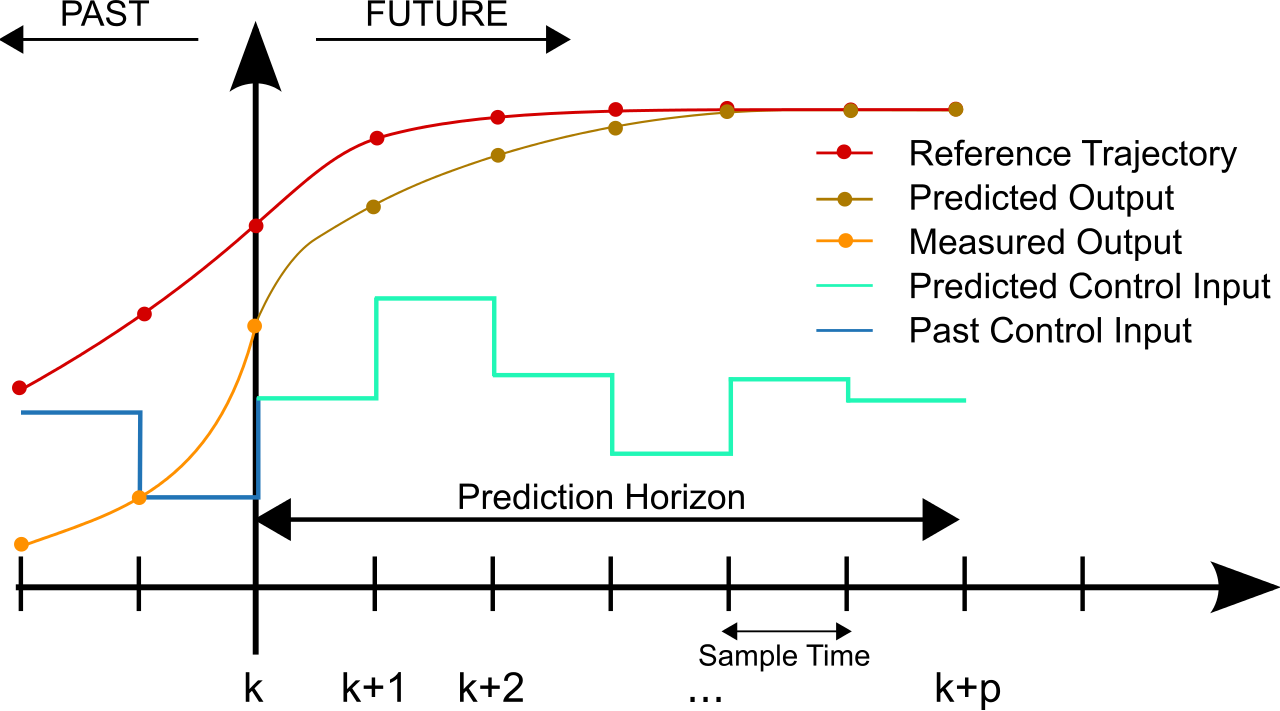
\includegraphics[width=0.7\textwidth]{MPC_scheme}
		\caption{A simple MPC diagram from the wikipedia page \cite{Wikipedia}}
		\label{fig:MPC diagram}
	\end{figure}
			
	\subsection{System}
		
	\subsection{Problem definition}
	The problem definition is based on \cite{Diehl2005}.
		\subsubsection{Problem form}
			The optimal control problem can be written as a non linear programming (NLP) problem  \eqref{eq:PANOC MPC form}. When solve the optimal inputs are obtained given a intial state $x_0$. Sometimes $x_0$ will be assumed to be part of the function f, just like the reference state and reference input. Which leads to the simplified equation, \eqref{eq:PANOC form} .
			\begin{equation}
				\underset{u}{\minimize} \  f(x_0,u) + g(u)
				\label{eq:PANOC MPC form}
			\end{equation}
			
			\begin{equation}
				\underset{u}{\minimize} \  f(u) + g(u)
				\label{eq:PANOC form}
			\end{equation}
		\subsubsection{Direct Single shoot}
			The direct single shoot definition with a predict horizon of N. Can be written as a NLP that is solved for $u=[u_0,u_1,... u_{N-1}]$. Each of the $u_k$ vectors is the inputs of the system at a particular time in the predict horizon. This means that the size of the vector u is the predict horizon multiplied with the dimension of the input .
			
			The cost on each step in the horizon is defined as \eqref{eq:single shot iteration cost}, this is called the stage cost.
			\begin{equation}
				\begin{aligned}
				& l_k(x_0,u) = &&  x_k^T Q x_k  +  u_k^T R u_k \\
				& \text{subject to}			&& x_0 = \bar{x} \\
				& 							&&  x_{n+1} = F_d(x_n,u_n), n=0...N-1
				\end{aligned}
				\label{eq:single shot iteration cost}
			\end{equation}
			
			The terminal cost is a special case of the stage cost, it is the last stage cost in the predict horizon. So if the Horizon is N, the terminal cost can be defined as \eqref{eq:single shot terminal cost}.
			
			\begin{equation}
				\begin{aligned}
					& l_N(x_0,u) = && x_N^TSx_N \\
					& \text{subject to}			&& x_0 = \bar{x} \\
					& 							&&  x_{n+1} = F_d(x_n,u_n), n=0...N-1
				\end{aligned}
				\label{eq:single shot terminal cost}
			\end{equation}
			
			The cost function $f(x_0,u)$ becomes \eqref{eq:single shot definition}, the sum of the stage costs and the terminal cost.
			
			\begin{equation}
				f(x_0,u) = \sum_{k=1}^{N-1} l_k(x_0,u) + l_N
				\label{eq:single shot definition}
			\end{equation}
			
			An other term can be added to \eqref{eq:single shot definition} to represent the obstacle avoidance. More on this later in the subsection on obstacles.
		\subsection{Direct Multiple shoot}
			The multiple shoot uses more initial information than just the initial inputs of the predict horizon. It requires an initial estimate of the intermediate states. These state estimates will be referred to as $x_i$ and the states derived from the estimate and its corresponding input will be referred to as $\bar{x_i}$. 
			
			Just as with the Single Shot, the goal is to find the optimal inputs $u_i$. However there are additional continuity conditions: $\bar{x_i} - x_{i+1} = 0$.
			
			\begin{equation}
				\bar{x_i} = F(x_i,u_i)
				\label{eq:}
			\end{equation}
			
			The continuity conditions are displayed in \eqref{eq:continuety condition multiple shot} and were not necessary in single shot, as there are no state estimates like $\bar{x}$. If the initial state estimates are relatively close to the solution, a significant speed increase can be accomplished. As more information can be incorporate into the problem.
			
			\begin{equation}
				\bar{x_i} - x_{i+1} = 0
				\label{eq:continuety condition multiple shot}
			\end{equation}
			
			The direct multiple shoot definition is formally defined as \eqref{eq:multiple shot cost}, and has an extra equality condition compared to the single shoot. The continuity conditions can be added as a soft constraints to the cost function. This is displayed in \eqref{eq:multiple shot cost with soft constraint} and will be used in the practical implementation.
			
			\begin{equation}
				\begin{aligned}
				L =  & \sum_{i=1}^{N} l(\bar{x_i},u_i) \\
				& \text{subject to}			&& \bar{x_i} = F(x_i,u_i) \\
				& 							&& \bar{x_i} - x_{i+1} = 0
				\end{aligned}
				\label{eq:multiple shot cost}
			\end{equation}
			
			\begin{equation}
			\begin{aligned}
			L =  & \sum_{i=1}^{N} l(\bar{x_i},u) + ||\bar{x_i} - x_{i+1}||\\
			& \text{subject to}			&& \bar{x_i} = F(x_i,u_i) \\
			\end{aligned}
			\label{eq:multiple shot cost with soft constraint}
			\end{equation}
			
		\subsection{Obstacle avoidance}
			The obstacle avoidance is based on the soft constraint definition described in \cite{AjaySathya2017}. It can be described as a set or an constraint.
			\subsubsection{As set}
				 obstacle can be defined as an open set, as illustrated by \eqref{eq:obstacle as open set}. It is defined by the intersection of a set of nonlinear inequalities.
				\begin{equation}
					O = \{ z \in \Re^d : h^i(z)>0,\ i \in N \}
					\label{eq:obstacle as open set}
				\end{equation}
				
			\subsubsection{As constraint}
				\begin{equation}
					[z]_+ =  \max\{0,z\}
				\end{equation}
				
				The statement $h(x)<0$ is equivalent to stating $[h(x)]_+=0$, so \eqref{eq:obstacle as open set} is equivalent to setting \eqref{eq:obstacle as equality} to zero.
				
				\begin{equation}
					\Phi_0(z) =  \frac{1}{2} \prod_{i=1}^m \Big( [h^i(z)]_+ \Big)^2
					\label{eq:obstacle as equality}
				\end{equation}
				
				The gradient of \eqref{eq:obstacle as equality} is define as \eqref{eq:obstacle as equality}
				
				\begin{equation}
					\nabla \Phi =
					\begin{cases}
						\sum_{i=1}^{m} h^i(z)\prod_{j \ne i} \Big( [h^j(z)]_+ \Big)^2 \nabla h^i(z)
						& x \in O \\
						0 & else
					\end{cases}
					\label{eq:derivative obstacle as equality}
				\end{equation}
			
			\subsubsection{Polyhedral obstacle}
				A simple obstacle example of such an obstacle is a polyhedral as defined in \eqref{eq:polyhedral constraint}.
				\begin{equation}
					\prod \Big([b_i - a_i^t z]_+ \Big)^2 = 0
					\label{eq:polyhedral constraint}
				\end{equation}
			
			\subsubsection{Obstacle as soft constraint}
				The obstacle avoidance is added as a soft constraint into the cost function. As demonstrated in \eqref{eq:derivative obstacle as equality}, this definition is two times differentiable and so this does not break the condition that the cost functions needs to be twice differentiable.
			
		\subsection{Input constraints}
			An other important aspect of a MPC problem is the input constraint. In practice inputs have to comply with the physical properties of the devices. For instance absurdly high or low input values might in theory lead to a fast solution, but are not feasible in practice.
			
			A major advantage of the PANOC algorithm is that it can take non linear or non convex constraints. As longs as the proximal mapping is analytically defined it is feasible. 
			
			A simple example is the indicator box function, which allows to set a maximum and minimum value on the inputs. (The indicator box function is defined in the appendix) Using the  indicator box function input constraint, demands that every feasible solution lies within the bounds of the user defined box.